\documentclass{beamer}
\usetheme{Boadilla} 
\setbeamercovered{invisible}
\setbeamertemplate{navigation symbols}{} 
%\useoutertheme{infolines} 

\usepackage[utf8]{inputenc}
\usepackage{graphicx}

\setbeamertemplate{frametitle continuation}{} 
\usepackage{subfigure}
\usepackage{caption}
\usepackage{bm}
\usepackage{epsfig}

\usepackage{amsmath}
\usepackage{xcolor,colortbl}

\usepackage{multicol}
\usepackage{wasysym}

\usepackage{hyperref}
\usepackage{float}

\usepackage{array}
\newcolumntype{L}[1]{>{\raggedright\let\newline\\\arraybackslash\hspace{0pt}}m{#1}}
\newcolumntype{C}[1]{>{\centering\let\newline\\\arraybackslash\hspace{0pt}}m{#1}}
\newcolumntype{R}[1]{>{\raggedleft\let\newline\\\arraybackslash\hspace{0pt}}m{#1}}

% deal with spaces in absolute paths

\usepackage[space]{grffile}
\graphicspath{{C:/Users/Yered/Dropbox/Harvard/Winter 2014/CdeC/Slides/Introduction/figures/}}

\usepackage[scaled]{helvet}
\usepackage[round]{natbib}


\begin{document}
\title[Introducción a la Expresión Genética]{Explorando el Transcriptoma con Datos de Expresi\'{o}n Gen\'{e}tica\\
\vspace{0.5cm}
Introducción a la Expresión Genética}
\author{Ingrid Rodr\'{i}guez\\
Yered Pita-Ju\'{a}rez}
\institute[CdeC M\'{e}rida]{}
\date{3/1/2015}


\begin{frame}
\titlepage
\end{frame}

\begin{frame}{Motivación}
\begin{itemize}
\item Mecanismos responsables de las características de los seres vivos
\item Ejemplos
\begin{itemize}
\item ¿Qué hace a los ratones y a los humanos diferentes?
\begin{figure}[H]
\centering
\begin{tabular}{cc}

\includegraphics[width=0.08\linewidth]{human.jpeg} &   
\includegraphics[width=0.15\linewidth]{mouse.png} \\
\end{tabular}
\end{figure}
\item ¿Porqué las células del hígado y las células del colon son diferentes?
\begin{figure}[H]
\centering
\begin{tabular}{cc}
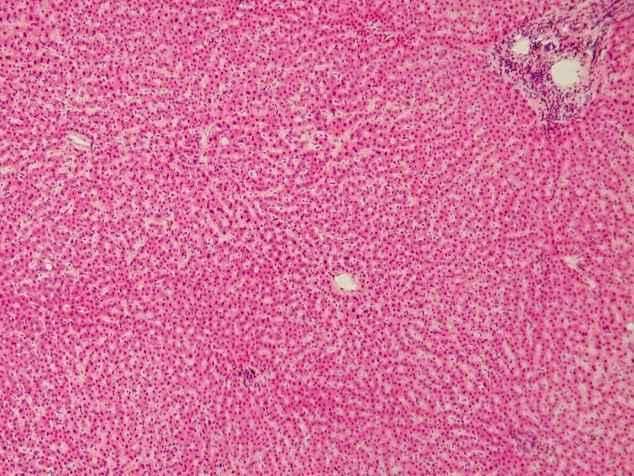
\includegraphics[width=0.25\linewidth]{human_liver_cells.jpg} &   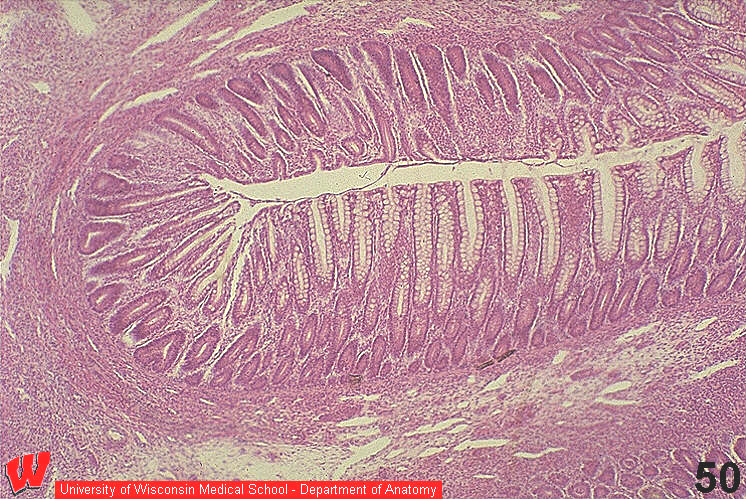
\includegraphics[width=0.27\linewidth]{colon_cells.jpg} \\
\end{tabular}
\end{figure}
\item ¿Porqué las celulas cancerosas viven más que las células normales?
\end{itemize}
\end{itemize}
\end{frame}

\begin{frame}{Motivación}
\begin{itemize}
\item La información contenida en las células se transmite a las siguientes generaciones
\item El ADN contiene las instrucciones necesarias para manufacturar y operar todos los componentes y procesos requeridos para la vida
\begin{figure}[H]
\centering
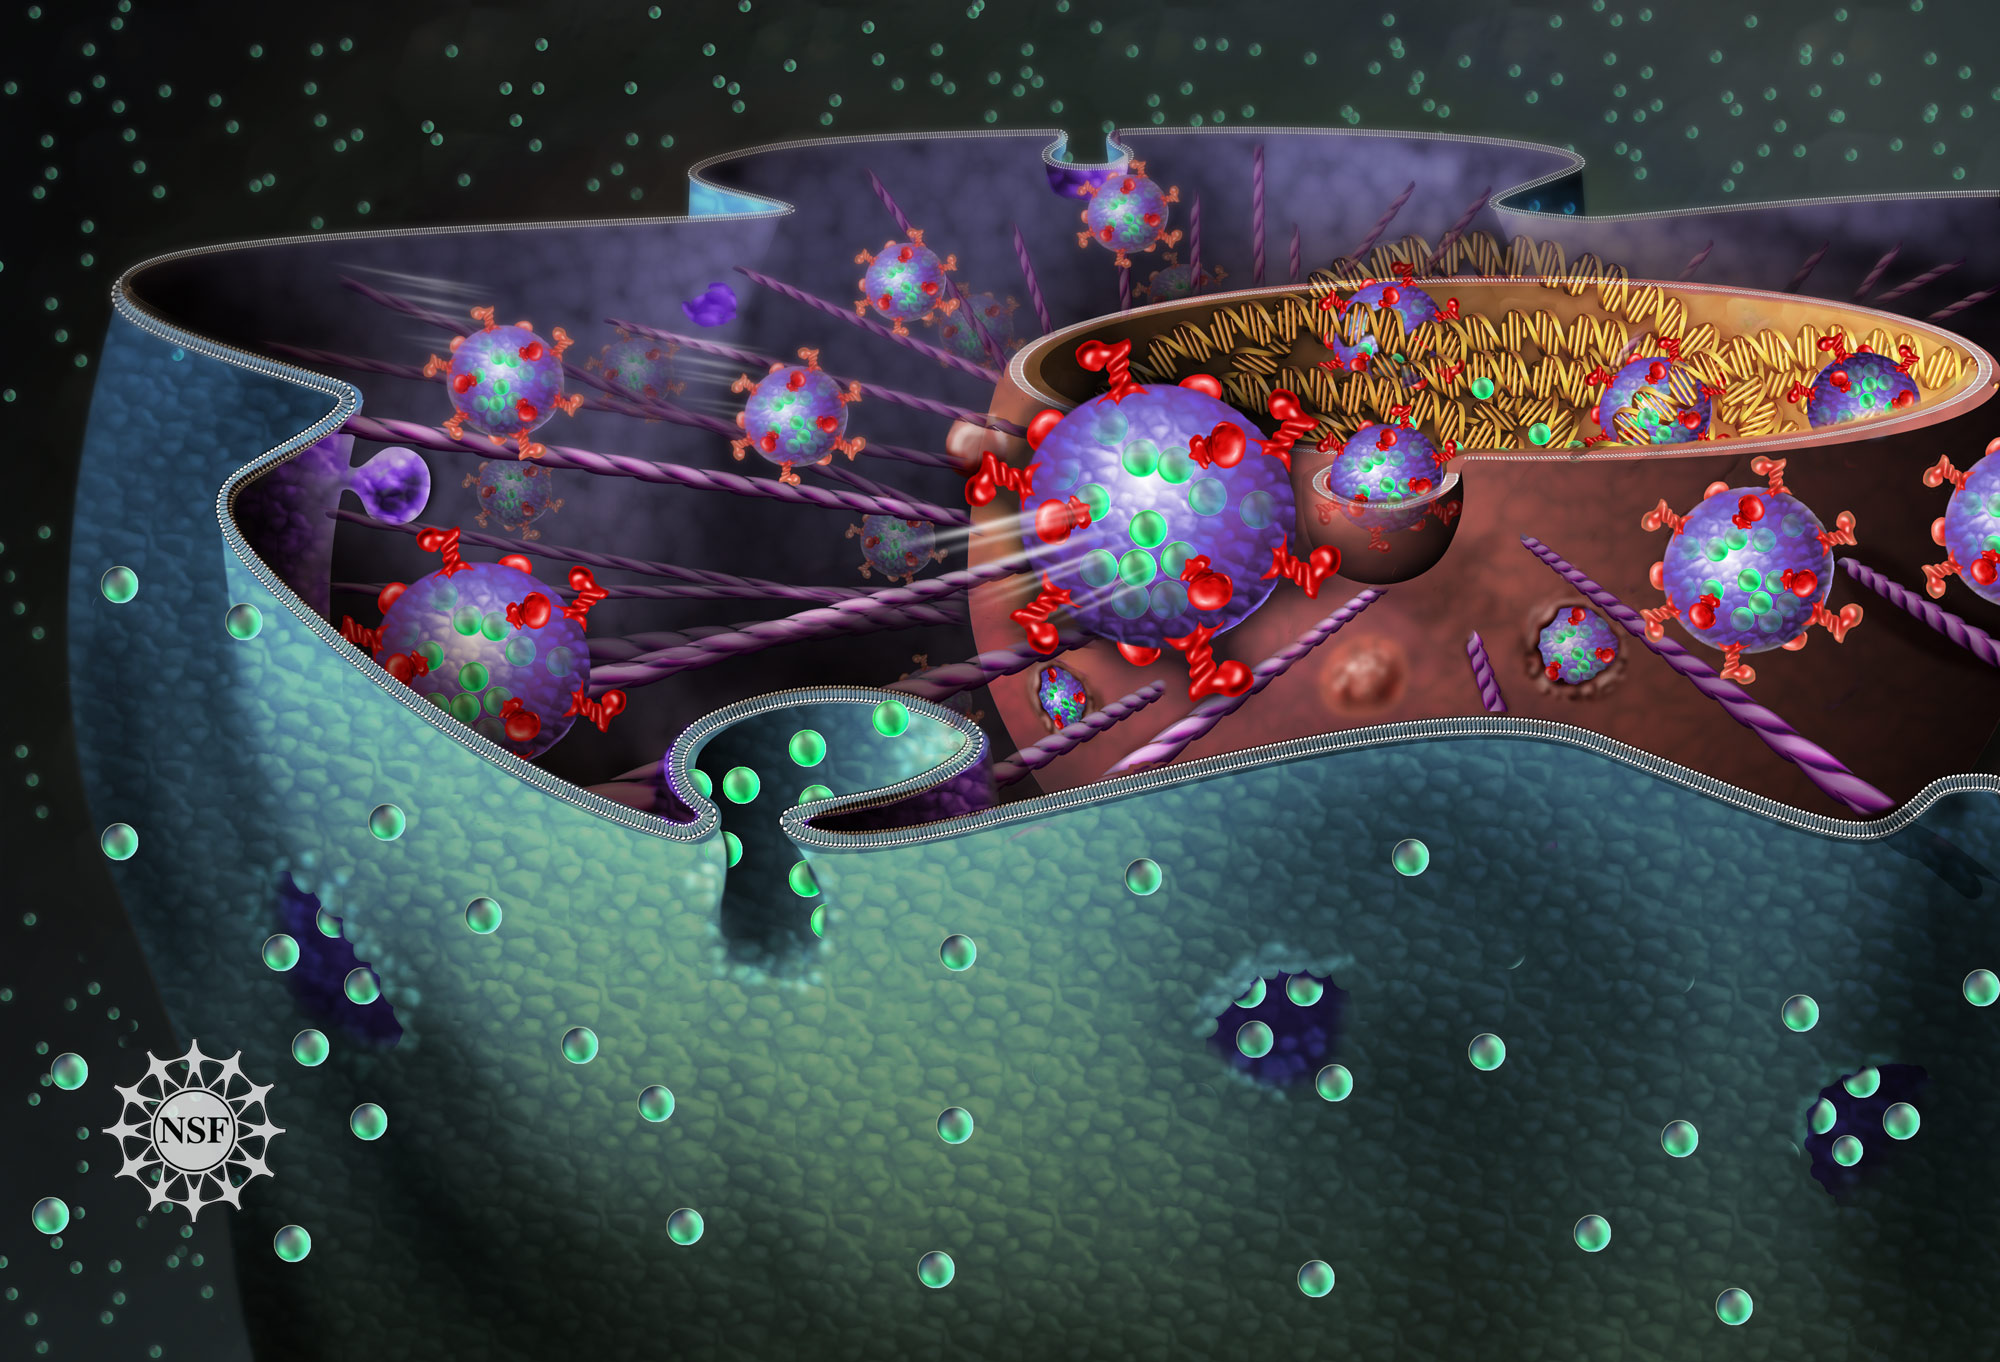
\includegraphics[scale=0.1]{Cell_nucleus.jpg}
\end{figure}
\end{itemize}
\end{frame}

%\begin{frame}{Motivación}
%\begin{itemize}
%\item Dogma Central: flujo de información
%\end{itemize}
%\begin{figure}[H]
%\centering
%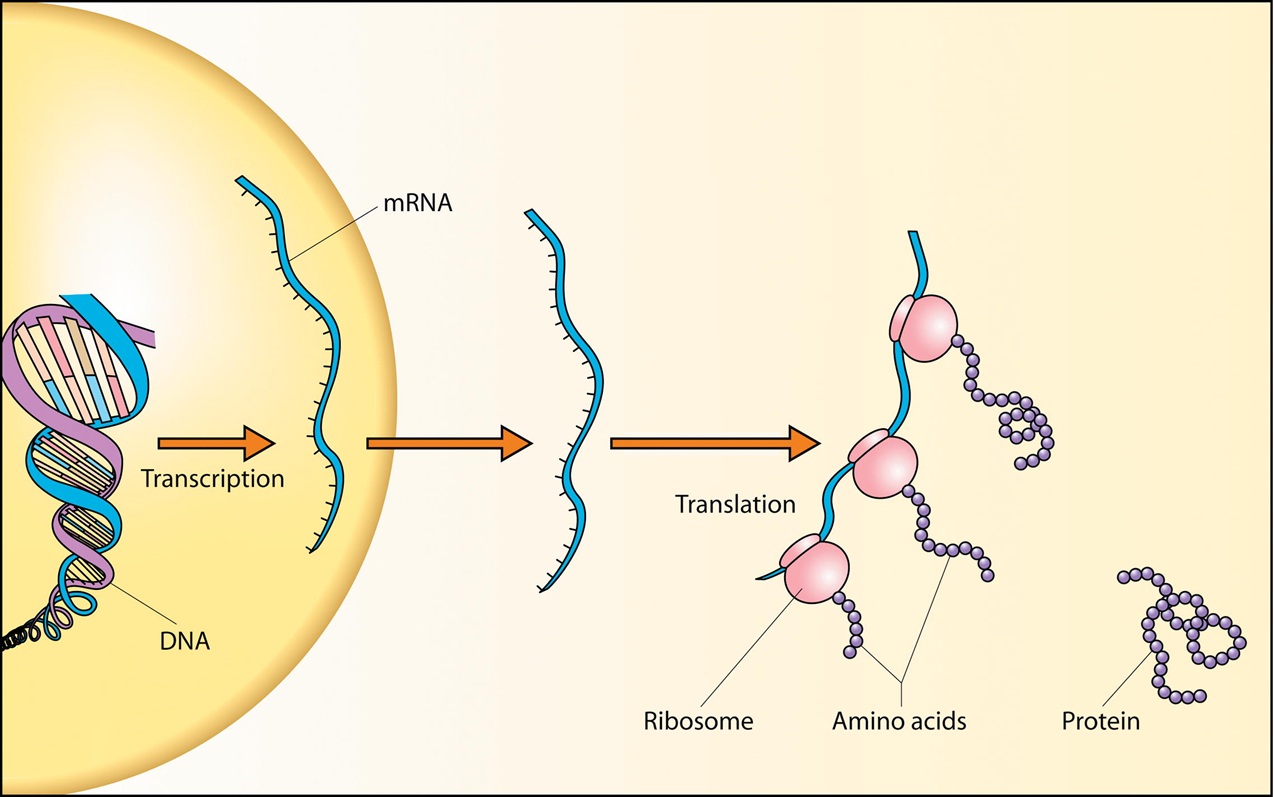
\includegraphics[scale=0.45]{dogma_diagram.png}
%\end{figure}
%\end{frame}



\begin{frame}{ADN}
\begin{columns}
    \begin{column}{0.47\textwidth}
\begin{itemize}
\item Ácido desoxirribonucleico (ADN)
\item Compuesto de 4 bases
\begin{itemize}
	\item Adenina (A)
	\item Timina (T)
	\item Citosina (C)
	\item Guanina (G)
\end{itemize}
\item Acoplamiento 
\begin{itemize}
	\item A-T
	\item G-C
\end{itemize}
\end{itemize}
    \end{column}
    \begin{column}{0.5\textwidth}
\begin{figure}[H]
\centering
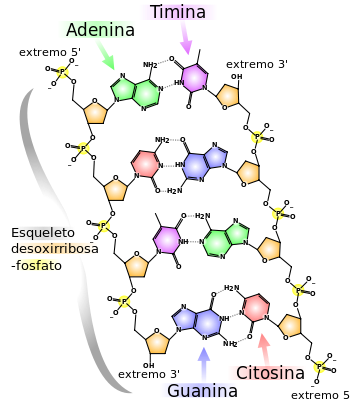
\includegraphics[scale=0.4]{DNA_structure.png}
\end{figure}
    \end{column}
\end{columns}
\end{frame}

\begin{frame}{ADN}
\begin{itemize}
\item El ADN es complementario
\end{itemize}
\begin{figure}
\centering
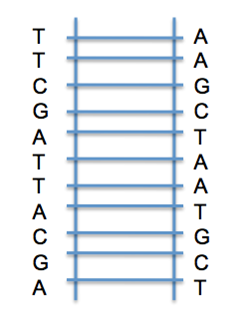
\includegraphics[scale=0.45]{DNA00.png}
\end{figure}
\end{frame}

\begin{frame}{ADN}
\begin{itemize}
\item El ADN es complementario
\end{itemize}
\begin{figure}
\centering
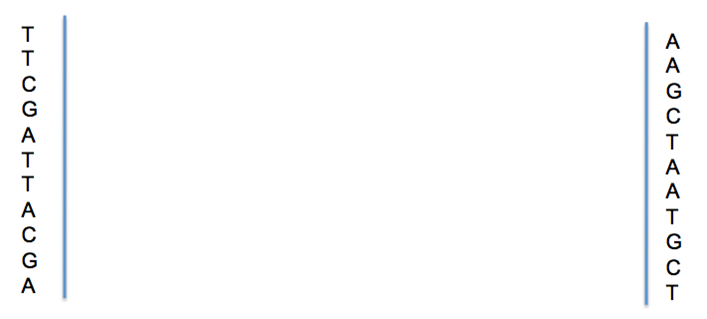
\includegraphics[scale=0.45]{DNA01.png}
\end{figure}
\end{frame}

\begin{frame}{ADN}
\begin{itemize}
\item El ADN es complementario
\end{itemize}
\begin{figure}
\centering
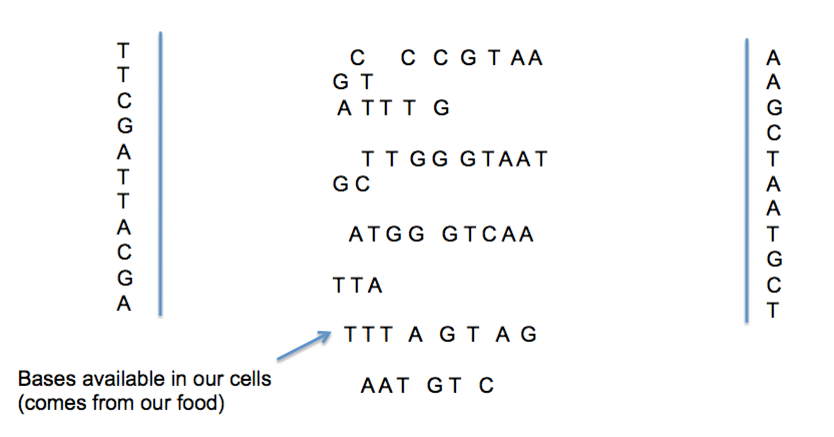
\includegraphics[scale=0.45]{DNA02.png}
\end{figure}
\end{frame}

\begin{frame}{ADN}
\begin{itemize}
\item El ADN es complementario
\end{itemize}
\begin{figure}
\centering
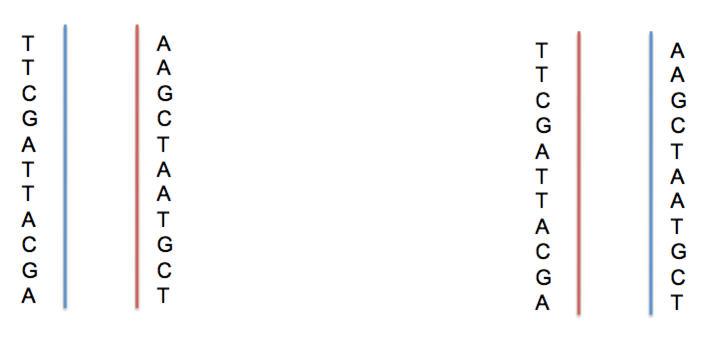
\includegraphics[scale=0.45]{DNA03.png}
\end{figure}
\end{frame}


\begin{frame}{ADN}
\begin{itemize}
\item El ADN es complementario
\end{itemize}
\begin{figure}
\centering
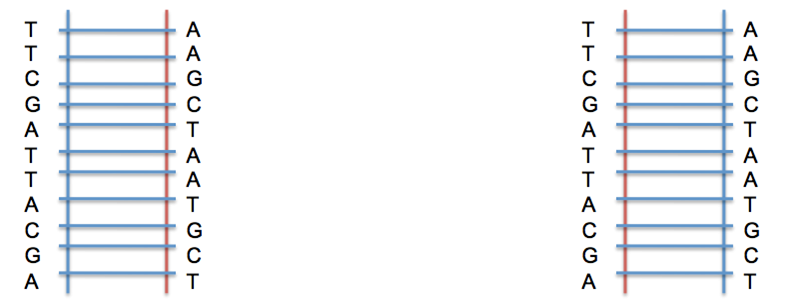
\includegraphics[scale=0.45]{DNA04.png}
\end{figure}
\end{frame}


\begin{frame}{Motivación}
\begin{itemize}
\item Dogma Central: flujo de información
\end{itemize}
\begin{figure}[H]
\centering
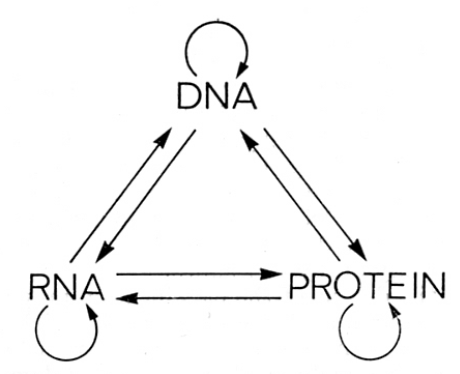
\includegraphics[scale=0.45]{dogma01.png}
\end{figure}
\end{frame}

\begin{frame}{Motivación}
\begin{itemize}
\item Dogma Central: flujo de información
\end{itemize}
\begin{figure}[H]
\centering
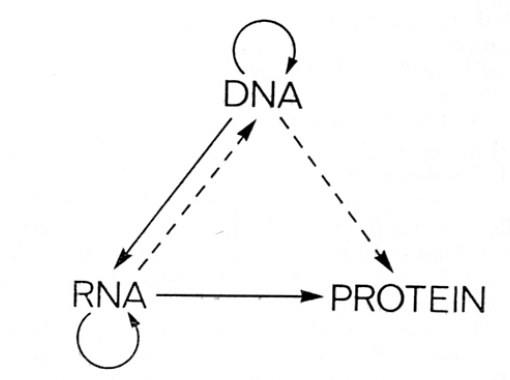
\includegraphics[scale=0.45]{dogma00.png}
\end{figure}
\end{frame}

\begin{frame}{Motivación}
\begin{itemize}
\item Dogma Central: flujo de información
\end{itemize}
\begin{figure}[H]
\centering
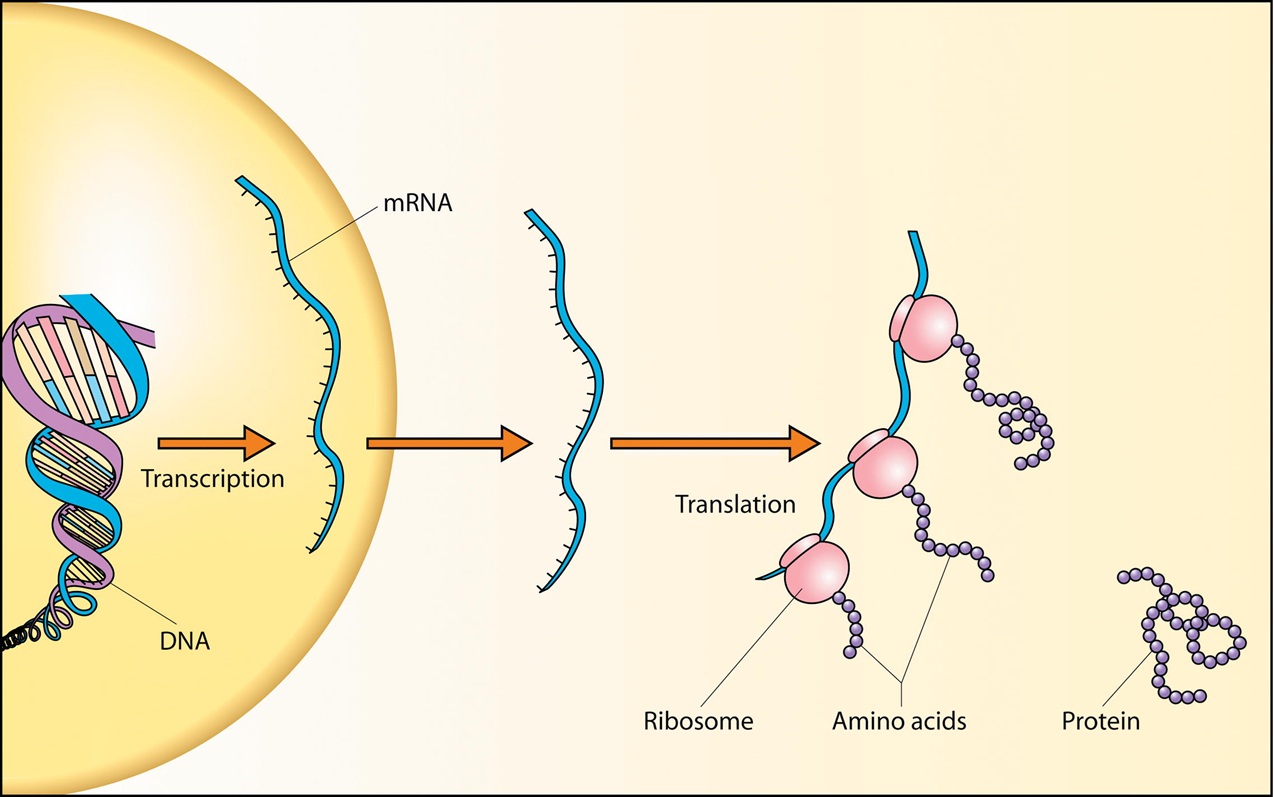
\includegraphics[scale=0.45]{dogma_diagram.png}
\end{figure}
\end{frame}



%\begin{frame}{Expresión Genética}
%\begin{itemize}
%\item Dogma Central: flujo de información
%\end{itemize}
%\begin{figure}[H]
%\centering
%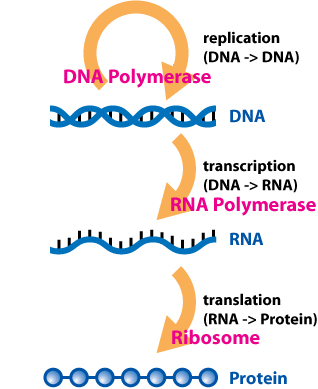
\includegraphics[scale=0.45]{central_dogma.jpg}
%\end{figure}
%\end{frame}


\begin{frame}{Gen}
\begin{figure}[H]
\centering
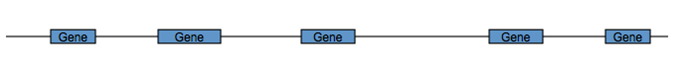
\includegraphics[scale=0.5]{gene00.png}
\end{figure}
\begin{figure}[H]
\centering
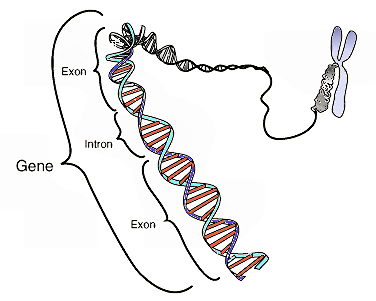
\includegraphics[scale=0.5]{gene01.png}
\end{figure}
\end{frame}

\begin{frame}{Transcripción}
\begin{figure}[H]
\centering
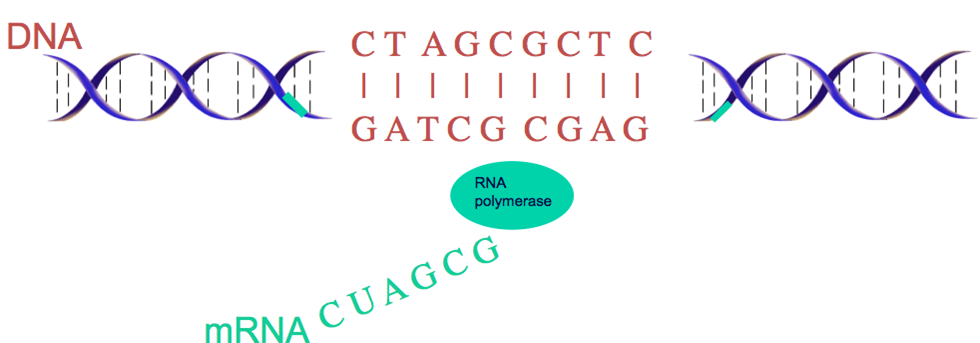
\includegraphics[scale=0.45]{gene02.png}
\end{figure}
\end{frame}

\begin{frame}{Traducción}
\begin{figure}[H]
\centering
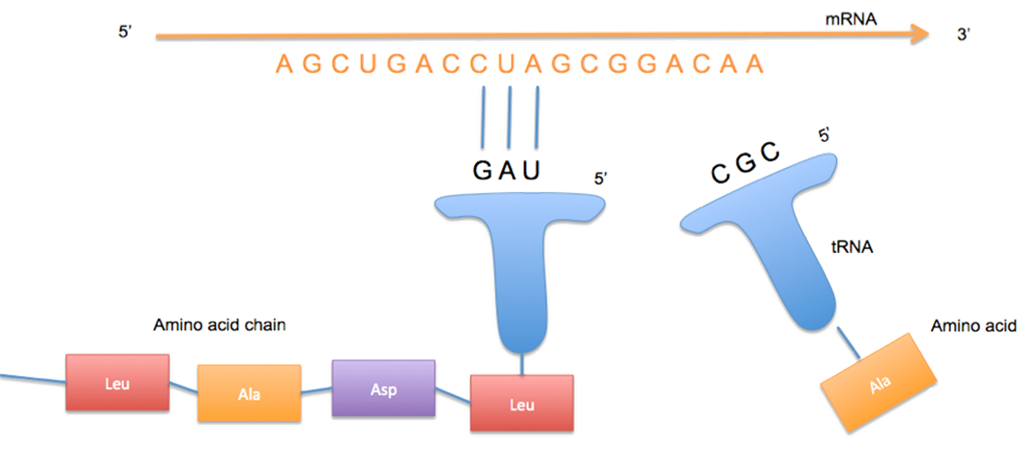
\includegraphics[scale=0.45]{gene03.png}
\end{figure}
\end{frame}

\begin{frame}{Transcriptoma}
\begin{itemize}
\item El conjunto de todas las moleculas de ARN en las células
\item Una célula no requiere de todas las proteínas, y las que usa las requiere en diferentes cantidades
%\item Expresión genética 
%\begin{itemize}
%	\item Expresión baja: produciendo pocas o nada de proteínas
%	\item Expresión alta: produciendo proteínas en abundancia
%\end{itemize}
%\item Medir niveles de ARN: expresión genética
\end{itemize}
\begin{figure}[H]
\centering
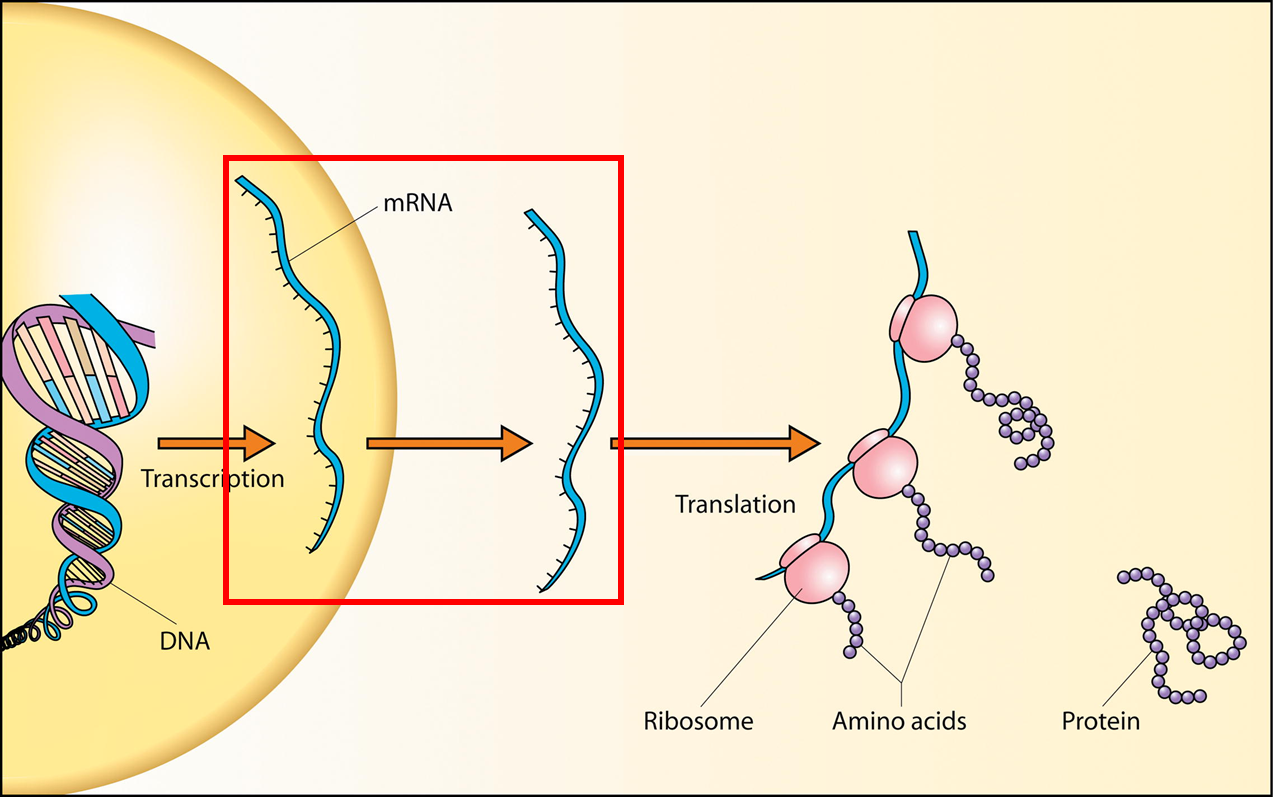
\includegraphics[scale=0.35]{transcriptome.png}
\end{figure}
\end{frame}

\begin{frame}{Transcriptoma}
\begin{itemize}
%\item El conjunto de todas las moleculas de ARN en las células
%\item Una célula no requiere de todas las proteínas, y las que usa las requiere en diferentes cantidades
\item Expresión genética 
\begin{itemize}
	\item Expresión baja: produciendo pocas o nada de proteínas
	\item Expresión alta: produciendo proteínas en abundancia
\end{itemize}
\item Medir niveles de ARN: expresión genética
\end{itemize}
\begin{figure}[H]
\centering
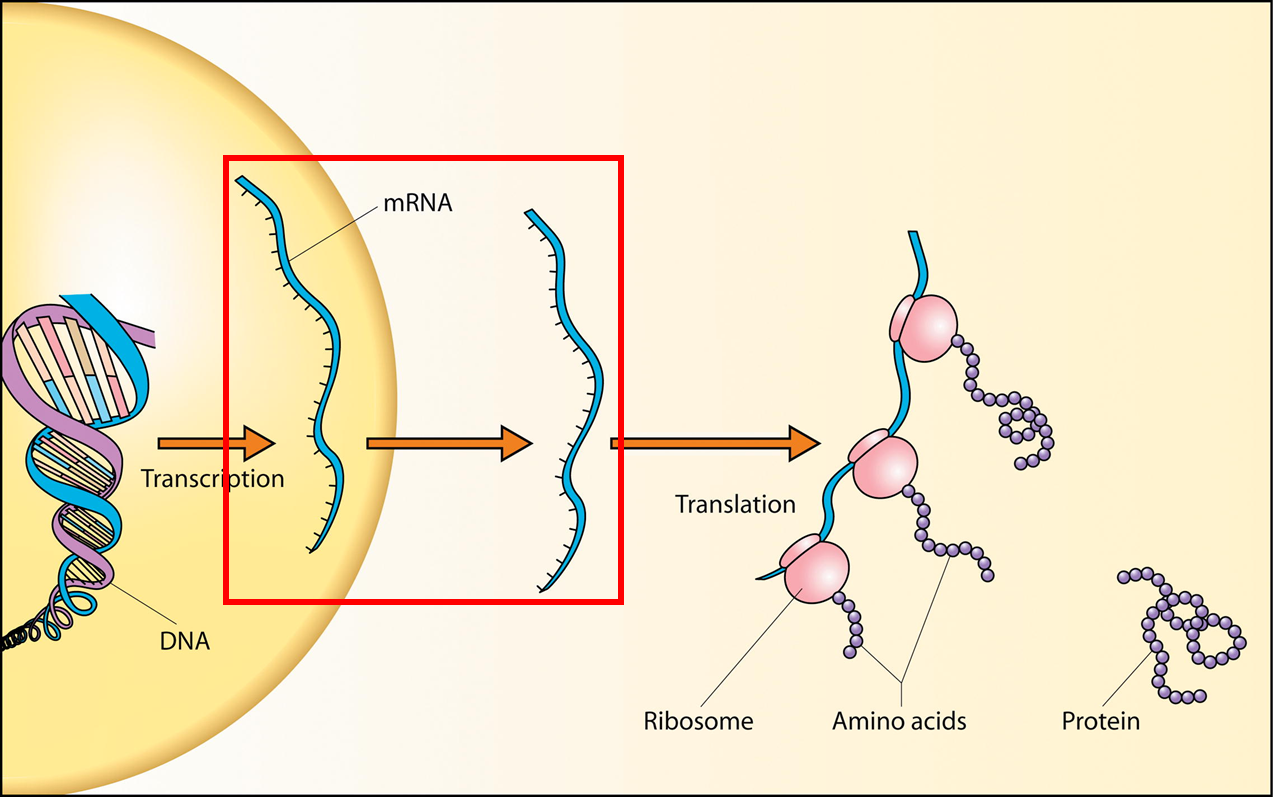
\includegraphics[scale=0.35]{transcriptome.png}
\end{figure}
\end{frame}

\end{document} 

